\documentclass[titlepage,a4paper,12pt]{article}

\usepackage[english,serbian]{babel}
\usepackage{mathptmx}
\usepackage{microtype}
\usepackage{graphicx}
\usepackage{wrapfig}
\usepackage{enumitem}
\usepackage{amsmath}
\usepackage{amsfonts}
\usepackage{listings}
\usepackage{xcolor}
\usepackage{placeins}
\usepackage{flafter}
\usepackage{enumitem}
\usepackage[normalem]{ulem}
\useunder{\uline}{\ulined}{}
\usepackage{pdfpages}
\usepackage{cancel}

\definecolor{codegreen}{rgb}{0,0.6,0}
\definecolor{codegray}{rgb}{0.5,0.5,0.5}
\definecolor{codepurple}{rgb}{0.58,0,0.82}
\definecolor{backcolour}{rgb}{0.95,0.95,0.92}

\lstdefinestyle{mystyle}{
	backgroundcolor=\color{backcolour},   
	commentstyle=\color{codegreen},
	keywordstyle=\color{magenta},
	numberstyle=\tiny\color{codegray},
	stringstyle=\color{codepurple},
	basicstyle=\ttfamily\footnotesize,
	breakatwhitespace=false,         
	breaklines=true,                 
	captionpos=b,                    
	keepspaces=true,                 
	numbers=left,                    
	numbersep=5pt,                  
	showspaces=false,                
	showstringspaces=false,
	showtabs=false,                  
	tabsize=2
}

\DeclareMathOperator{\sinc}{sinc}

\lstset{style=mystyle}

\renewcommand{\lstlistingname}{Kod}
\renewcommand{\lstlistlistingname}{Lista \lstlistingname ova}

\usepackage{tikz}
\usetikzlibrary{math}

\begin{document}	
	\tikzmath{
		integer \godina;
		\godina = 2020;
		integer \indeks;
		\indeks = 260;
		integer \varsum;
		\varsum = \indeks + \godina;
		integer \digsumindeks;
		\digsumindeks = \indeks / 1000 + Mod(\indeks / 100,10) + Mod(\indeks/10,10) + Mod(\indeks,10);
		integer \digsumgodina;
		\digsumgodina = \godina / 1000 + Mod(\godina / 100,10) + Mod(\godina/10,10) + Mod(\godina,10);
		integer \digsum;
		\digsum = \digsumindeks + \digsumgodina;
		integer \Pval;
		\Pval = Mod(\varsum, 4);
		integer \Qval;
		\Qval = Mod(\digsum, 4);
	}
	
	\begin{titlepage}
		\begin{center}
			\vspace*{1cm}
			
			\Huge
			\textbf{Signali i sistemi}\\
			\LARGE
			\textbf{Domaći 2}
			
			\vspace{1cm}
			\Large
			
			Branislav Đumić\\
			Br. indeksa: 0\indeks/\godina
			\vfill
			
			%\begin{figure*}[ht]
			%	\centering
			%	\includegraphics[width=\textwidth]{Images/indeks.png}
			%\end{figure*}
			\vfill
			Parametri
			
			\vspace{0.25cm}
			\large
			P = \Pval, Q = \Qval
			
		\end{center}
	\end{titlepage}
	\normalfont
	\tableofcontents
	\clearpage
	\includepdf[pages={2}]{tekstzadatka.pdf}
	\clearpage
	\begin{center}
		\LARGE\textbf{Rešenje}
	\end{center}

	\indent U daljem tekstu FDM sistem za paralelni prenos iz zadatka nazivaćemo Sistem. Sistem se sastoji od više filtara, sabirača i modulatora. Funkcije filtara će biti opisane u narednoj sekciji. Sistem sadrži dva modulatora kojima se moduliše i demoduliše jedan od prenošenih signala. Sabirač služi za kombinovanje prenošenih signala, kako bi se oni mogli prenositi istim kanalom.

	\section{Filtri FDM sistema za paralelni prenos}
	Prvo ćemo imenovati različite filtre u Sistemu. Usvajamo notaciju za obeležavanje filtara:
	\begin{equation*}
		X\big[TF\big] \; \Big| \;\omega_x\;:\;x(t) \rightarrow y(t).
	\end{equation*}
	Pri ovoj notaciji $X$ je ime funkcije frekvencijskog odziva filtra $X(j\omega)$, $TF$ je tip filtra, $\omega_x$ je granična učestanost filtra, dok su signali $x(t)$ i $y(t)$ ulazni, odnosno izlazni, signal filtra. Pri ovoj notaciji filtri koje imamo u Sistemu su:
	\begin{alignat*}{3}
		&H_{n_1}&\big[NF\big] &\Big| \;\omega_{u1}\;&:\; y_1(t) \rightarrow y_1^n(t)\\
		&H_{n_2}&\big[NF\big] &\Big| \;\omega_{u2}\;&:\; y_2(t) \rightarrow y_2^n(t)\\
		&H_{kv}&\big[NF\big] &\Big| \;\omega_{kv}\;&:\; y_T(t) \rightarrow y_R(t)\\
		&H_{Rb_1}&\big[NF\big] &\Big| \;\omega_{i1}\;&:\; y_R(t) \rightarrow y_1^r(t)\\
		&H_{Rb_2}&\big[PO\big] &\Big| \;\omega_{o2}\;&:\; y_R(t) \rightarrow y_2^b(t)\\
		&H_{d_2r_2}&\big[NF\big] &\Big| \;\omega_{i2}\;&:\; y_2^d(t) \rightarrow y_2^r(t)
	\end{alignat*}

	$H_{n_1}$ je ulazni filtar Sistema. Njegova uloga je uklanjanje slabije izraženih učestanosti iz spektra ulaznog signala $y_1(t)$. Ovime se omogućava prenošenje signala $y_1(t)$ i $y_2(t)$ bez njihovog mešanja, tako što će sekanalom veze prenositi samo korisne, odnosno najizraženije, učestanosti.
	
	\smallskip
	$H_{n_2}$ je, takođe, ulazni filtar Sistema. Vrši istu funkciju kao i filtar $H_{n_1}$, ali nad signalom $y_2(t)$.
	
	\smallskip
	$H_{kv}$ je filtar kojim modeluje kanal veze. Prenošeni signal $y_T(t)$ prenosi informacije na nižim ušestanostima, tako da je potrebno sprečiti smenje na ovim učestanostima. Na višim učestanostima nema značajnih informacija. Kanal veze se treba modelovati tako da što manje utiše na prenošeni signal. Zbog ovoga ga, kanal veze modelujemo filtrom niskih učestanosti. 
	
	\smallskip
	$H_{Rb_1}$ prihvata prenešeni signal i iz njegovog spektra izdvaja učestanosti koje nose korisne o prvobitnom signalu $y_1(t)$. Pod korisnim inforacijam smatraju se učestanosti prvobitno izdvojene ulaznim filtrima.
	
	\smallskip
	$H_{Rb_2}$ takođe prihvata prenešeni signal, ali iz njega izdvaja spektar učestanosti koji predstavlja signal $y_2(t)$. Pošto je pre prenošenja signal bio modulisan, njegov spektar se nalazi levo i desno u odnosu na spektar ulaznog signala $y_2(t)$. Zbog ovoga je ovaj filtar propusnik opsega; potrebno je prigušiti spektar učestanosti signala $y_1(t)$, kao i učestanosti viših od onih na kojima se prenosi signal $y_2(t)$.
	
	\smallskip
	$H_{d_2r_2}$ je filtar koji uklanja "duplikate" spektra početnog signala, tj. one učestanosti koje su se pojavile u spektru usled postupaka modulacije i demodulacije.
	\clearpage
	
	\section{Određivanje frekvencijskih spektara signala $y_1(t)$ i $y_2(t)$}
	\indent Na osnovu zadatih parametara mogu se odretiti analitički oblici signala $y_1(t)$ i $y_2(t)$:
	\begin{gather}
		y_1(t) = \sin(2000\pi t)e^{-100t}u(t)\\
		y_2(t) = \big[u(t)-u(t-0.0005)\big]-
		\big[u(t-0.0005)-u(t-0.001)\big]
	\end{gather}
	\indent Frekvencijski spektri ulaznih signala, $Y_1(j\omega)$ i $Y_2(j\omega)$ jednaki su njihovim Furijeovim transformacijama:
	\begin{flalign}
		Y_1(j\omega) = \mathcal{F}\big\{y_1(t)\big\}\\
		Y_2(j\omega) = \mathcal{F}\big\{y_2(t)\big\}
	\end{flalign}
	\subsection{Frekvencijski spektar signala $y_1(t)$}
	\indent Kako bi lakše odredili frekvencijski spektar signala $y_1(t)$, napisaćemo ga kao proizvod signala $y_{11}(t)$ i $y_{12}(t)$:
	\begin{flalign}
		y_1(t) &= y_{11}(t) \cdot y_{12}(t)\\
		y_{11}(t) &= \sin(2000\pi t)\\
		y_{12}(t) &= e^{-100t}u(t)
	\end{flalign}
	Odredimo sada spektar signala $Y_1(j\omega)$. Prema osobinama Furijeove transformacije imamo:
	\begin{equation}
		Y_1(j\omega) = \mathcal{F}\big\{y_1(t)\big\} = \mathcal{F}\big\{y_{11}(t)\cdot y_{12}(t)\big\} =
		\frac{1}{2\pi}\mathcal{F}\big\{y_{11}(t)\big\}*\mathcal{F}\big\{y_{12}(t)\big\}\label{eq:prodtoconv}
	\end{equation}
	Odredimo sada spektar signala $y_{11}(t)$:
	\begin{flalign*}
		Y_{11}(j\omega) &= \mathcal{F}\big\{y_{11}(t)\big\} = \mathcal{F}\big\{\sin(2000\pi t)\big\} = \mathcal{F}\Bigg\{ \frac{e^{j2000\pi t} - e^{-j2000\pi t} }{2j} \Bigg\}\\
		Y_{11}(j\omega)  &= \frac{1}{2j} \Big(
		\mathcal{F}\big\{e^{j2000\pi t}\big\}-
		\mathcal{F}\big\{e^{-j2000\pi t}\big\}\Big)\\
		Y_{11}(j\omega) &=\frac{1}{2j} \Big(
		2\pi\delta(\omega-2000\pi) - 2\pi\delta(\omega+2000\pi)\Big)
	\end{flalign*}
	Konačan izraz za spekar signala $y_{11}(t)$je:
	\begin{equation}
		Y_{11}(j\omega) =\frac{\pi}{j} \Big(
		\delta(\omega-2000\pi) - \delta(\omega+2000\pi)\Big)\label{eq:Y11}
	\end{equation}
	Izračunajmo spektar signala $y_{12}(t)$:
	\begin{flalign*}
		Y_{12}(j\omega) &= \mathcal{F}\big\{y_{12}(t)\big\} = \int_{-\infty}^{+\infty}e^{-100t}u(t)e^{-j\omega t}dt = \int_0^{+\infty}e^{-100t}e^{-j\omega t}dt\\
		Y_{12}(j\omega) &= \int_0^{+\infty}e^{-(100+j\omega)t} = -\frac{1}{100+j\omega}\Big[e^{-100t}e^{-j\omega t}\Big] \Bigg|_0^{+\infty}\\
		Y_{12}(j\omega) &= -\frac{1}{100+j\omega }
		\Bigg[\lim_{\tau\to+\infty}\Big(e^{-100\tau}e^{-j\omega\tau }\Big) - \cancelto{1}{\lim_{\tau\to\ +\infty}\Big(e^{-100\cdot\tau}e^{-j\omega \cdot \tau}\Big)} \Bigg]\\
		Y_{12}(j\omega) &= -\frac{1}{100+j\omega }
		\Bigg[\cancelto{0}{\lim_{\tau\to+\infty}\Big(e^{-100\tau}\Big)}\lim_{\tau\to+\infty}\Big(e^{-j\omega\tau }\Big) - 1\Bigg]
	\end{flalign*}
	Konačan izraz za spektar signala $y_{12}(t)$:
	\begin{equation}
			Y_{12}(j\omega) =\frac{1}{100+j\omega }\label{eq:Y12}
	\end{equation}
	Iz izraza \eqref{eq:prodtoconv}, \eqref{eq:Y11} i \eqref{eq:Y12} imamo za spektar signala $y_1(t)$, $Y_1(j\omega)$:
	\begin{align*}
		Y_1(j\omega) &= \frac{1}{2\pi}Y_{11}(j\omega)*Y_{11}(j\omega)\\
		Y_1(j\omega) &= \frac{1}{2\cancel{\pi}}\int_{-\infty}^{+\infty}
		\frac{\cancel{\pi}}{j} \Big(
		\delta(\lambda-2000\pi) - \delta(\lambda+2000\pi)\Big)
		\frac{1}{100+j(\omega-\lambda)}d\lambda\\
		Y_1(j\omega) &= \frac{1}{2j}\Bigg(\int_{-\infty}^{+\infty}
		\frac{\delta(\lambda-2000\pi)}{100+j(\omega-\lambda)}d\lambda
		-\int_{-\infty}^{+\infty}
		\frac{\delta(\lambda+2000\pi)}{100+j(\omega-\lambda)}d\lambda
		\Bigg)
	\end{align*}
	Konačno se za frekvencijski spektar $Y_1(j\omega)$ dobija izraz:
	\begin{equation}
		Y_1(j\omega) = \frac{1}{2j}\Bigg(
		\frac{1}{100+j(\omega-2000\pi)} -
		\frac{1}{100+j(\omega+2000\pi)}
		\Bigg)\label{eq:Y1Final}
	\end{equation}
	Sređivanjem izraza \eqref{eq:Y1Final} dobijamo:
	\begin{equation*}
		Y_1(j\omega) = \frac{2000\pi}{100^2-\omega^2+2000^2\pi^2+j200\omega}
	\end{equation*}
	Odavde možemo odrediti amplitudsku frekvencijsku karakteristiku signala $y_1(t)$:
	\begin{equation}
		|Y_1(j\omega)| = \frac{2000\pi}{\sqrt{(100^2-\omega^2+2000^2\pi^2)^2+200^2\omega^2}}
	\end{equation}
	\clearpage
	Kada se nacrta grafik amplitudske frekvencijske karakteristike dobijmao sledeću sliku:
	\begin{figure}[ht]
		\centering
		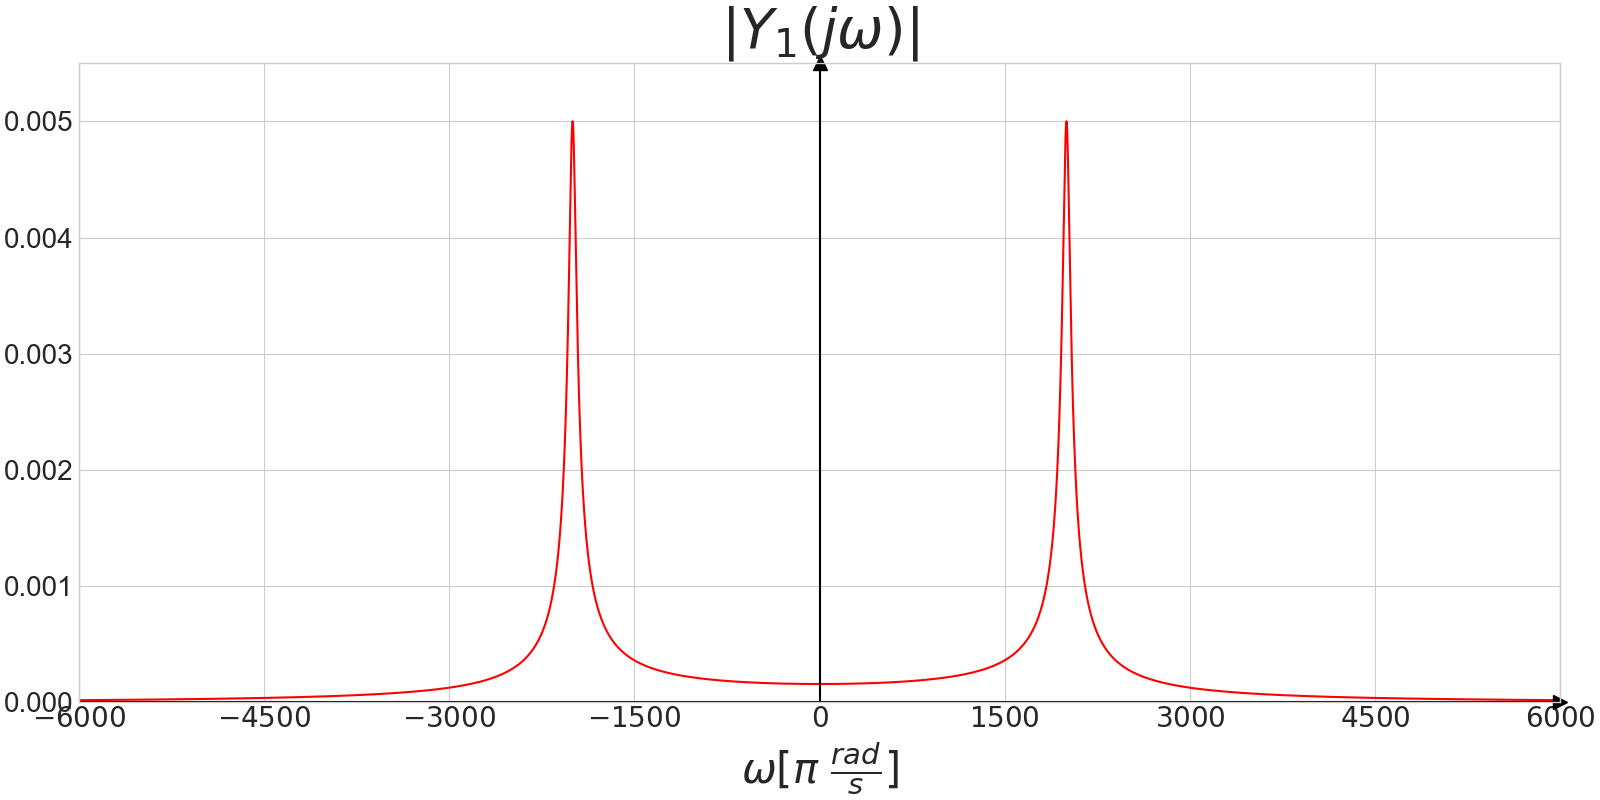
\includegraphics[width=\textwidth]{Images/AmpY1.png}
		\caption{Amplitudski spektar $Y_1(j\omega)$}\label{fig:AmpY1}
	\end{figure}
	\FloatBarrier
	\clearpage

	\subsection{Frekvencijski spektar signala $y_2(t)$}
	\indent Kako bi lakše odredili frekvencijski spektar signala $y_2(t)$, napisaćemo ga kao razliku signala $y_{21}(t)$ i $y_{22}(t)$:
	\begin{flalign}
		y_2(t) &= y_{21}(t) - y_{22}(t)\\
		y_{21}(t) &= u(t)-u(t-0.0005)\\
		y_{22}(t) &= u(t-0.0005)-u(t-0.001)
	\end{flalign}
	Za signale $y_{21}(t)$ i $y_{22}(t)$ važi:
	\begin{equation*}
		y_22(t) = y_21(t-0.0005)
	\end{equation*}
	Iz osobina furijeove transformacije važe sledeće relacije:
	\begin{gather}
		Y_2(j\omega) = \mathcal{F}\big\{y_2(t)\big\} = \mathcal{F}\big\{y_{21}(t) - y_{22}(t)\big\}=
		\mathcal{F}\big\{y_{21}(t)\big\} - \mathcal{F} \big\{y_{22}(t)\big\}\label{eq:Y2asdiff}\\
		Y_2(j\omega) = Y_{21}(j\omega) - Y_{22}(j\omega)\\
		Y_{22}(j\omega) = \mathcal{F}\big\{y_1(t-0.0005)\big\}=
		e^{-j\omega 0.0005}Y_{21}(j\omega)\label{eq:Y22overY21}
	\end{gather}
	Izračunajmo spektar signala $y_{21}(t)$:
	\begin{align}
		Y_{21}(j\omega) &= \int_{-\infty}^{+\infty}\Big(u(t)-u(t-0.0005)\Big)e^{-j\omega t}dt = \int_{0}^{0.0005}e^{-j\omega t}dt\notag\\
		Y_{21}(j\omega) &= -\frac{1}{j\omega}\cdot e^{-j\omega t}\Big|_0^{0.0005} = \frac{1-e^{-j\omega 0.0005}}{j\omega}\label{eq:Y21}
	\end{align}
	Iz jednačina \eqref{eq:Y2asdiff}, \eqref{eq:Y22overY21} i \eqref{eq:Y21} možemo sračunati konačan izraz za spektar $Y_2(j\omega)$:
	\begin{flalign*}
		Y_2(j\omega) &= Y_{21}(j\omega) - e^{-j\omega 0.0005}Y_{21}(j\omega)\\
		Y_2(j\omega) &= \frac{1}{j\omega}\Big(1-e^{-j\omega 0.0005}\Big)^2\\
		Y_2(j\omega) &= \frac{1}{j\omega}\Big(e^{-j\omega 0.00025}\Big(e^{j\omega 0.00025}-e^{-j\omega 0.00025}\Big)\Big)^2\\
		Y_2(j\omega) &= \frac{1}{j\omega}e^{-j\omega 0.0005}\Big(2j\cdot\sin(0.00025\omega)\Big)^2\\
		Y_2(j\omega) &= -\frac{4}{j\cancel{\omega}}e^{-j\omega 0.0005}\cdot\sin^2(0.00025\omega)\cdot\frac{0.00025^2\omega^{\cancelto{1}{2}}}{0.00025^2\omega^2}
	\end{flalign*}
	Konačno za frekvencijski spektar $Y_2(j\omega)$ dobijamo:
	\begin{equation}
		Y_2(j\omega) = 2.5\cdot10^{-7} j\omega e^{-j\omega 0.0005}\cdot\sinc^2(0.00025\omega)\label{eq:Y2Final}
	\end{equation}
	Iz jednačine \eqref{eq:Y2Final} možemo odrediti amplitudsku frekvencijsku karakteristiku signala $y_2(t)$:
	\begin{equation}
		|Y_2(j\omega)|= 2.5\cdot10^{-7}|\omega|\sinc^2(0.00025\omega)\label{eq:Y2FinalABS}
	\end{equation}
	Kada se nacrta grafik amplitudske frekvencijske karakteristike dobijmao sledeću sliku:
	\begin{figure}[ht]
		\centering
		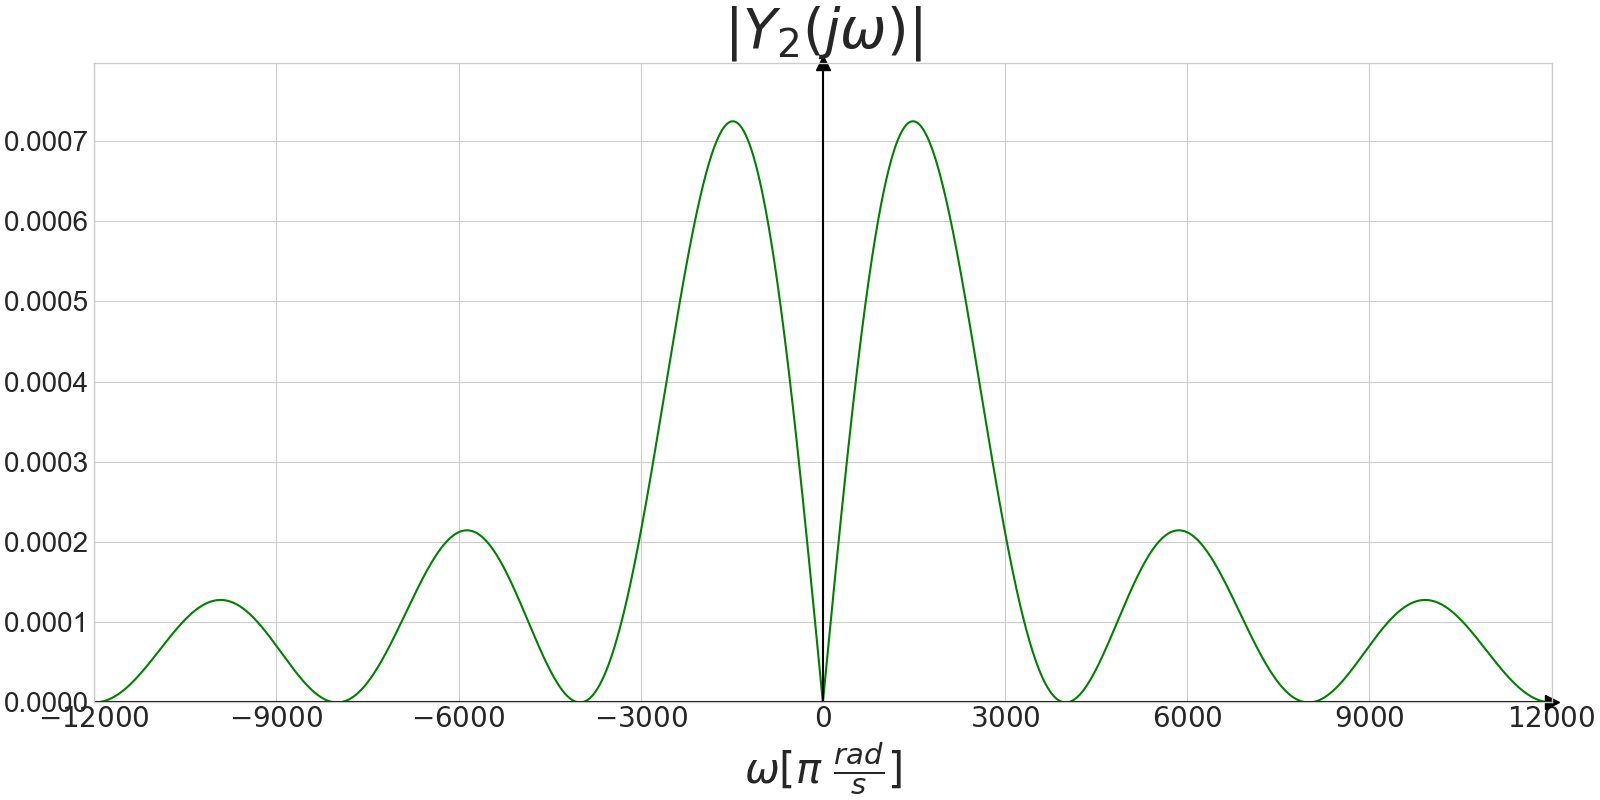
\includegraphics[width=\textwidth]{Images/AmpY2.png}
		\caption{Amplitudski spektar $Y_2(j\omega)$}\label{fig:AmpY2}
	\end{figure}
	\FloatBarrier
	\clearpage
	
	\section{Izbor graničnih učestanosti filtara i učestanosti nosioca $f_c$}
	Izaberimo i obrazložimo učestanosti svih filtara u Sistemu i granične učestanosti nosioca. Na osnovu usvojenih graničnih učestanosti možemo odrediti izraze za amplitudske frekvencijske karakteristike svih filtara sistema.
	\bigskip
	
	Na osnovu slike \ref{fig:AmpY1}. vidimo da je najznačajniju komponentu signala $y_1(t)$ moguće predstaviti učestanostima do $4000\pi \frac{rad}{s}$, tako da za učestanost filtra $H_{n1}$ biramo $\omega_{u1} = 4000\pi \frac{rad}{s}$.
	\begin{equation}
		|H_{n1}(j\omega)| = \left\{
		\begin{array}{ll}
			1& |\omega| < \omega_{u1} \\
			0& |\omega| > \omega_{u1}
		\end{array}\right.
	\end{equation} 
	
	\bigskip
	Na osnovu slike \ref{fig:AmpY2}. vidimo da je najveći deo spektra signala $y_2(t)$ obuhvaćen učestanostima manjim od $\omega_g = 8000\pi \frac{rad}{s}$,
	tako da za učestanost filtra $H_{n2}$ biramo $\omega_{u2} = 8000\pi \frac{rad}{s}$. Čak i ovim izborom, značajan deo učestanosti biva izostavljen, ali projetovanje filtara sa većim propusnim opsegom bi bilo nepraktično.
	\begin{equation}
		|H_{n2}(j\omega)| = \left\{
		\begin{array}{ll}
			1& |\omega| < \omega_{u2} \\
			0& |\omega| > \omega_{u2}
		\end{array}\right.
	\end{equation} 
	
	\bigskip
	Učestanost nosioca $f_c$ treba da odaberemo tako da ne dođe do mešanja signala $y_1^n(t)$ i $y_2^m(t)$ pri njihovom sabiranju. Kako bi to postigli, modulacijom signala $y_2^n(t)$ potrebno je pomeriti njegov spektar za $\omega_c = \omega_{u1} + \omega_{u2} = 12000\pi\frac{rad}{s}$. Kako je $f_c = \frac{\omega_c}{2\pi}$, dobijamo da je učestanost nosioca $f_c = 6000Hz$.
	
	\bigskip
	Granična učestanost filtra $H_{Rb_1}$ treba da bude jednaka učestanosti filtra  $H_{n1}$, pošto oni treba da izoluju isti opseg učestanosti. Dakle, $\omega_{i1} = 4000\pi \frac{rad}{s}$. 
	\begin{equation}
		|H_{Rb1}(j\omega)| = \left\{
		\begin{array}{ll}
			1& |\omega| < \omega_{i1} \\
			0& |\omega| > \omega_{i1}
		\end{array}\right.
	\end{equation} 
	
	\bigskip
	Filtar $H_{Rb_2}$ ima dve granične učestanosti, s obzirom da je on filtar propusnik opsega. Ovaj filtar bi trebalo da izoluje modulisan signal $y_2^m(t)$ tj. razdvoji ga od signala $y_1^n(t)$. Donja granična učestanost, $\omega_{o2d}$ jednaka je gornjoj graničnoj učestanosti filtra $H_{n1}$, jer na njoj prestaju učestanosti kojima se prenosi signal $y_1^n(t)$. Dakle, imamo da je	$\omega_{o2d} = 4000\pi \frac{rad}{s}$. Gornja granična učestanost  $\omega_{o2g}$ jednaka je najvišoj učestanosti na kojoj prenosimo informacije.  Kako je signal koji izdvajamo nastao modulacijom, njegov imamo $\omega_{o2g} =\omega_{u_2}+\omega{c} = 20000\pi \frac{rad}{s}$.
	\begin{equation}
		|H_{Rb_2}(j\omega)| = \left\{
		\begin{array}{ll}
			0& |\omega| < \omega_{o2d}\\
			1& \omega_{o2d} < |\omega| < \omega_{o2g}] \\
			0& |\omega| > \omega_{o2g}
		\end{array}\right.
	\end{equation} 
	
	\bigskip
	Granična učestanost filtra $H_{d_2r_2}$ treba da bude jednaka učestanosti filtra  $H_{n2}$, pošto oni treba da izoluju isti opseg učestanosti. Dakle, $\omega_{i1} = 8000\pi \frac{rad}{s}$. 
	\begin{equation}
		|H_{d_2r_2}(j\omega)| = \left\{
		\begin{array}{ll}
			1& |\omega| < \omega_{i2} \\
			0& |\omega| > \omega_{i2}
		\end{array}\right.
	\end{equation} 
	
	\bigskip
	Granična učestanost filtra $H_{kv}$, kanala veze, mora biti dovoljno visoka da ne dođe do oštećenja signala $y_T(t)$ pri prenosu. Potrebno je obuhvatiti čitav spektar ovog signala. Imamo da je $\omega_{kv} = \omega_{u1}+2\cdot\omega_{u2} = 20000\pi\frac{rad}{s}$.
	\begin{equation}
		|H_{kv}(j\omega)| = \left\{
		\begin{array}{ll}
			1& |\omega| < \omega_{kv} \\
			0& |\omega| > \omega_{kv}
		\end{array}\right.
	\end{equation} 
	
	\clearpage
	
	\section{Amplitudske karakteristike signala sistema}
	\subsection{Signal $y_1^n(t)$}
	Signal $y_1^n(t)$ nastaje propuštanjem signala $y_1(t)$ kroz filtar $H_{n1}$. 
	Usled filtracije, signal $y_1^n(t)$ sadrži samo učestanosti manje od $\omega_{u1} = 4000\pi\frac{rad}{s}$. Znamo da je izlazni signal filtra $H_{n1}$, $y_1^n(t)$, jednak konvoluciji ulaznog signala $y_1(t)$ i impulsnog odziva filtra $h_{n1}(t)$, odnosno
	\begin{equation}
		y_1^n(t) = y_1(t) * h_{n1}(t).
	\end{equation}
	Prema osobinama Furijeove transformacije,u frekvencijskom domenu imamo:
	\begin{gather}
		Y_1^N(j\omega) = Y_1(j\omega)\cdot H_{n1}(j\omega)\\
		|Y_1^N(j\omega)| = |Y_1(j\omega)|\cdot |H_{n1}(j\omega)|\notag\\
		|Y_1^N(j\omega)| = \left\{\begin{array}{lll}
			|Y_1(j\omega)| &|\omega| < \omega_{u1} \\
			0 &|\omega| > \omega_{u1}
		\end{array}\right.
	\end{gather}
	Na donjoj slici možemo videti amplitudksi spektar signala $y_1^n(t)$.
	\begin{figure*}[ht]
		\centering
		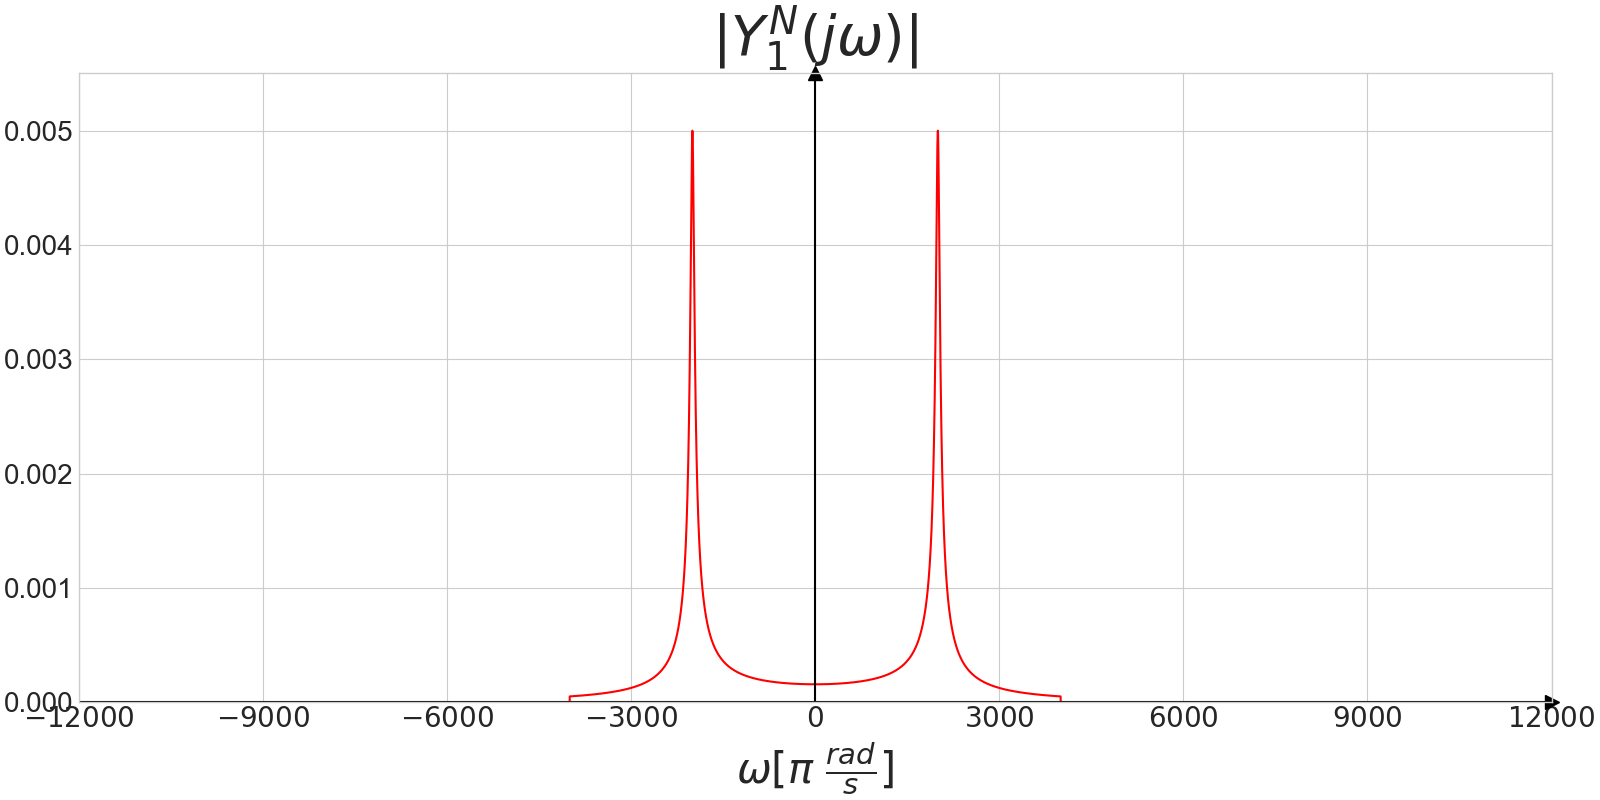
\includegraphics[width=\textwidth]{Images/AmpY1N.png}
		\caption{Amplitudski spektar $|Y_1^N(j\omega)|$}\label{fig:AmpY1N}
	\end{figure*}
	\FloatBarrier
	\clearpage

	\subsection{Signal $y_2^n(t)$}
	Signal $y_2^n(t)$ nastaje propuštanjem signala $y_2(t)$ kroz filtar $H_{n2}$. 
	Usled filtracije, signal $y_2^n(t)$ sadrži samo učestanosti manje od $\omega_{u2} = 8000\pi\frac{rad}{s}$. Znamo da je izlazni signal filtra $H_{n2}$, $y_2^n(t)$, jednak konvoluciji ulaznog signala $y_2(t)$ i impulsnog odziva filtra $h_{n2}(t)$, odnosno
	\begin{equation}
		y_2^n(t) = y_2(t) * h_{n2}(t).
	\end{equation}
	Prema osobinama Furijeove transformacije,u frekvencijskom domenu imamo:
	\begin{gather}
		Y_2^N(j\omega) = Y_2(j\omega)\cdot H_{n2}(j\omega)\\
		|Y_2^N(j\omega)| = |Y_2(j\omega)|\cdot |H_{n2}(j\omega)|\notag\\
		|Y_2^N(j\omega)| = \left\{\begin{array}{lll}
			|Y_2(j\omega)| &|\omega| < \omega_{u2} \\
			0 &|\omega| > \omega_{u2}
		\end{array}\right.
	\end{gather}
	Na donjoj slici možemo videti amplitudksi spektar signala $y_2^n(t)$.
	\begin{figure*}[ht]
		\centering
		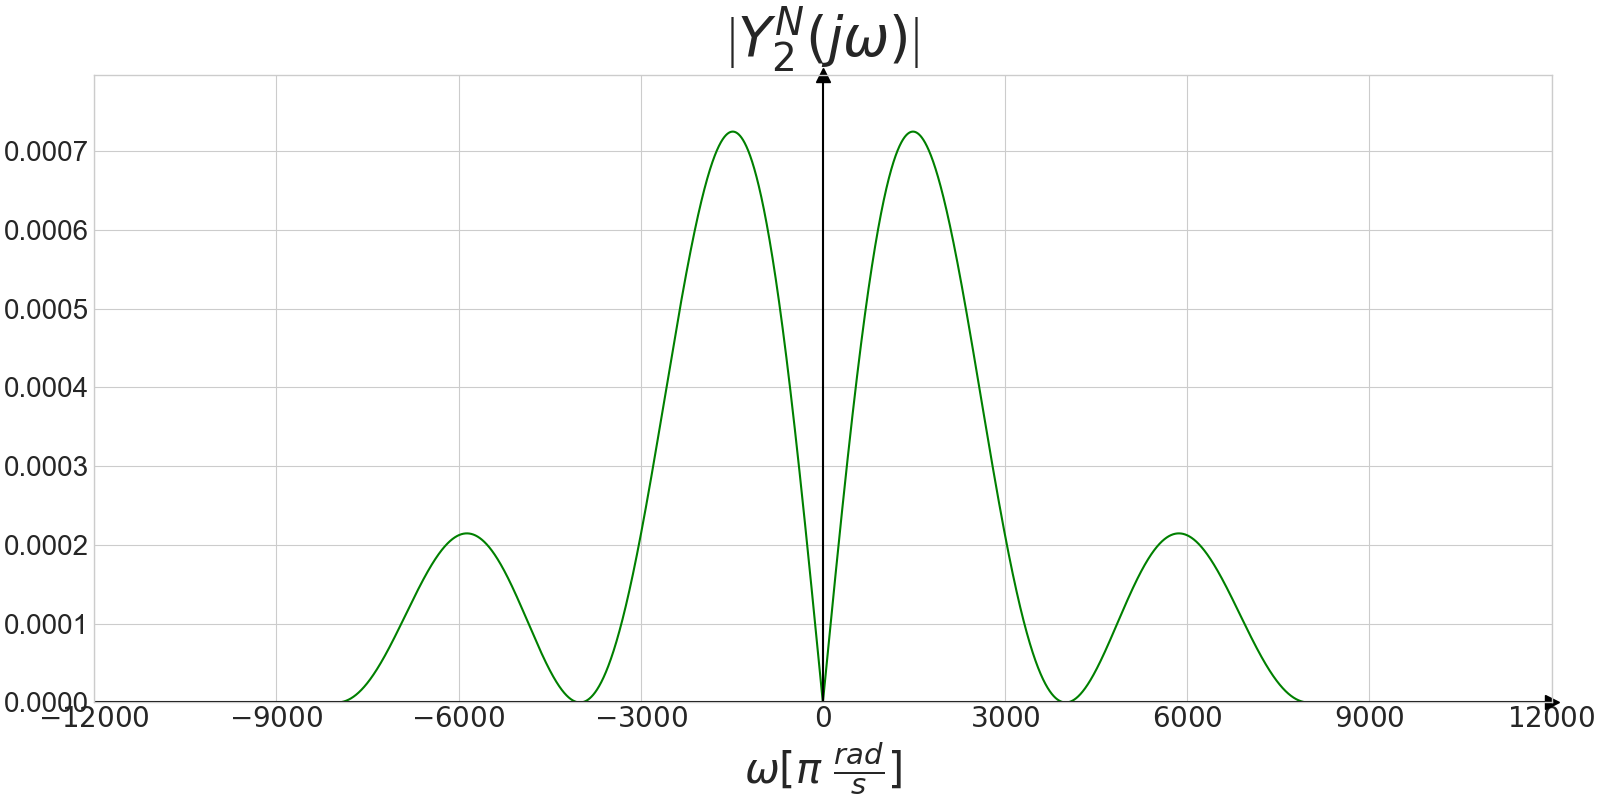
\includegraphics[width=\textwidth]{Images/AmpY2N.png}
		\caption{Amplitudski spektar $|Y_2^N(j\omega)|$}\label{fig:AmpY2N}
	\end{figure*}
	\FloatBarrier
	\clearpage
	
	\subsection{Signal $y_2^m(t)$}
	Signal $y_2^m(t)$ nastaje modulisanjem signala $y_2^n(t)$ sinusoidom $\cos(2\pi f_c\cdot t)$. Dakle u vremenskom domenu imamo:
	\begin{equation}
		y_2^m(t) = y_2^n(t)\cos(2\pi f_c\cdot t).
	\end{equation}
	Prelaskom u frekvencijski domen dobijamo sledeće:
	\begin{equation}
		Y_2^M(j\omega) = \frac{1}{2\pi} Y_2^N(j\omega)*\mathcal{F}\big\{\cos(2\pi f_c\cdot t)\big\}
	\end{equation}
	Odredimo frekvencijski spektar signala $y_2^m(t)$.
	\begin{align*}
		Y_2^M(j\omega) &= \frac{1}{2\pi} Y_2^N(j\omega)*\mathcal{F}\Bigg\{ \frac{e^{j2\pi f_c t}+e^{-j2\pi f_c t}}{2} \Bigg\}\\
		Y_2^M(j\omega) &= \frac{1}{4\pi} Y_2^N(j\omega)*\Bigg(\mathcal{F}\big\{e^{j2\pi f_c t} \big\}
		+\mathcal{F}\big\{e^{-j2\pi f_c t} \big\}\Bigg)\\
		Y_2^M(j\omega) &= \frac{1}{4\pi}Y_2^N(j\omega)*\Big( 2\pi\delta(\omega-2\pi f_c) + 2\pi\delta(\omega+2\pi f_c)\Big)\\
		Y_2^M(j\omega) &= \frac{1}{2}Y_2^N(j\omega)*\Big(\delta(\omega-2\pi f_c) + \delta(\omega+2\pi f_c)\Big)\\
		Y_2^M(j\omega) &= \frac{1}{2}\int_{-\infty}^{+\infty}Y_2^N(j\lambda)\Big(\delta(\omega-\lambda-2\pi f_c) + \delta(\omega-\lambda+2\pi f_c)\Big)d\lambda\\
		Y_2^M(j\omega) &= \frac{1}{2}\Bigg[Y_2^N(j\lambda)\Big|_{\lambda = \omega - 2\pi f_c} + Y_2^N(j\lambda)\Big|_{\lambda = \omega + 2\pi f_c}\Bigg]
	\end{align*}
	Konačno se za frekvencijski spektar dobija:
	\begin{equation}
		Y_2^M(j\omega) = \frac{1}{2}\Big[Y_2^N\big(j(\omega - 2\pi f_c)\big) + Y_2^N\big(j(\omega + 2\pi f_c)\big)\Big]
	\end{equation}
	Sada možemo odrediti amplitudski spektar signala $y_2^m(t)$:
	\begin{equation}
		|Y_2^M(j\omega)| = \left\{
		\begin{array}{clrrl}
			0& \omega \in (&-\infty,& -20000\pi) \\
			\frac{1}{2}|Y_2^N\big(j(\omega+2\pi f_c)\big)|& \omega \in (&-20000\pi,& -4000\pi) \\
			0& \omega \in (&-4000\pi,& 4000\pi) \\
			\frac{1}{2}|Y_2^N\big(j(\omega-2\pi f_c)\big)|& \omega \in (&4000\pi,& 20000\pi) \\
			0& \omega \in (&20000\pi,& +\infty)
		\end{array}\right.
	\end{equation}
	\clearpage
	Na sledećoj slici možemo videti amplitudski spektar signala $y_2^m(t)$:
	\begin{figure*}[ht]
		\centering
		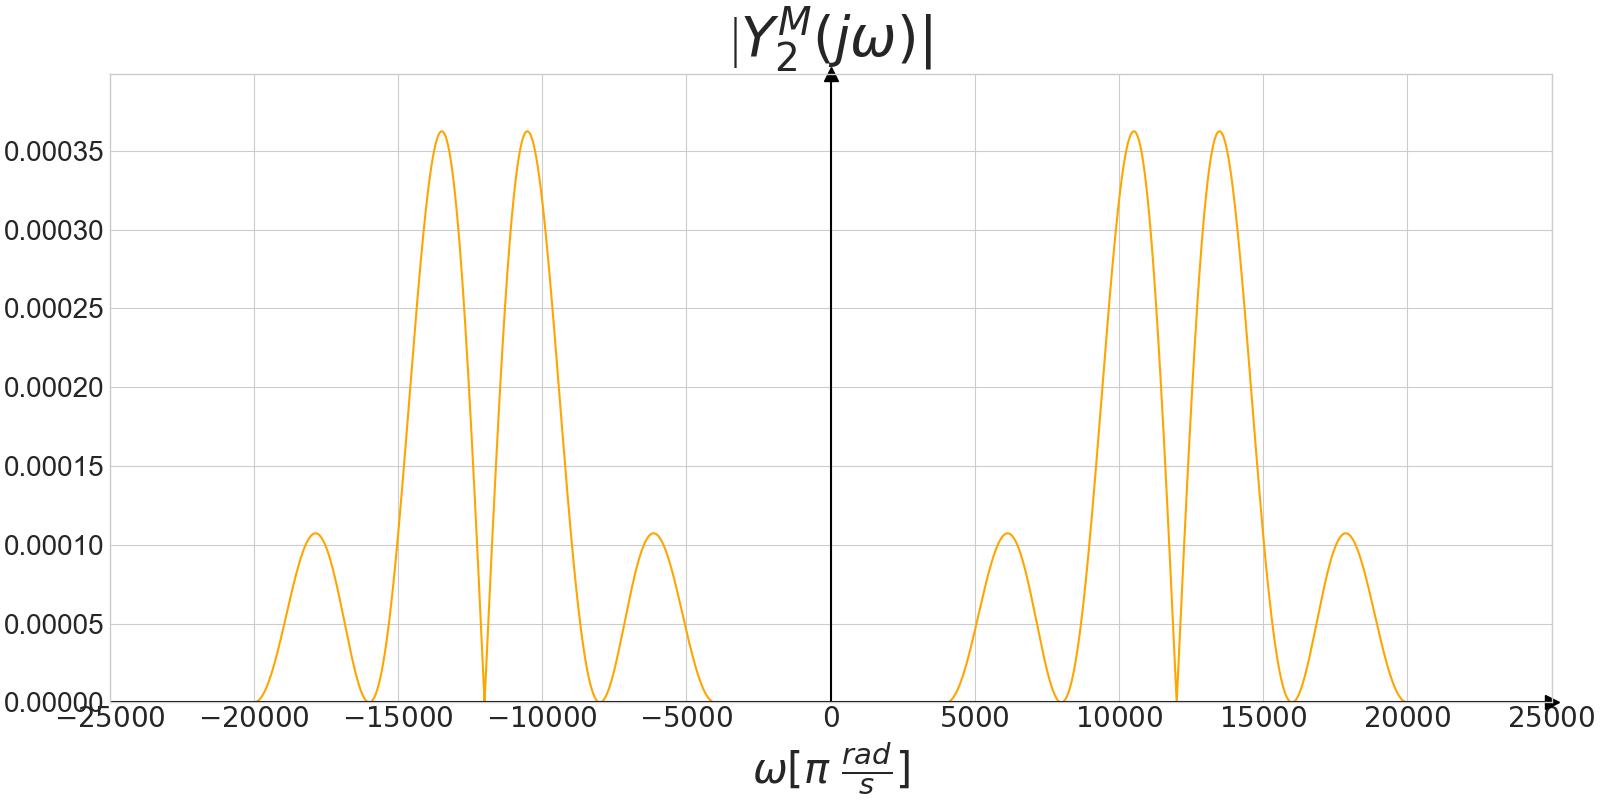
\includegraphics[width=\textwidth]{Images/AmpY2M.png}
		\caption{Amplitudski spektar $|Y_2^M(j\omega)|$}\label{fig:AmpY2M}
	\end{figure*}
	\FloatBarrier
	\clearpage
	
	\subsection{Signal $y_T(t)$}
	Signal $y_T(t)$ je signal koji se prenosi putem kanala veze. Nastaje sabiranjem signala $y_1^n(t)$ i $y_2^m(t)$. Dakle imamo:
	\begin{gather}
		y_T(t) = y_1^n(t) + y_2^m(t)\\
		Y_T(j\omega) = Y_1^N(j\omega) + Y_2^M(j\omega)\\
		|Y_T(j\omega)| = \left\{
		\begin{array}{rlrrl}
			0& \omega \in (&-\infty,& -20000\pi) \\
			\frac{1}{2}|Y_2^N\big(j(\omega+2\pi f_c)\big)|& \omega \in (&-20000\pi,& -4000\pi) \\
			|Y_1^N\big(j\omega\big)|& \omega \in (&-4000\pi,& 4000\pi) \\
			\frac{1}{2}|Y_2^N\big(j(\omega+2\pi f_c)\big)|& \omega \in (&4000\pi,& 20000\pi) \\
			0& \omega \in (&20000\pi,& +\infty)
		\end{array}\right.
	\end{gather}
	Na sledećoj slici vidimo amplitudski sprektar signala $y_T(t)$:
	\begin{figure*}[ht]
		\centering
		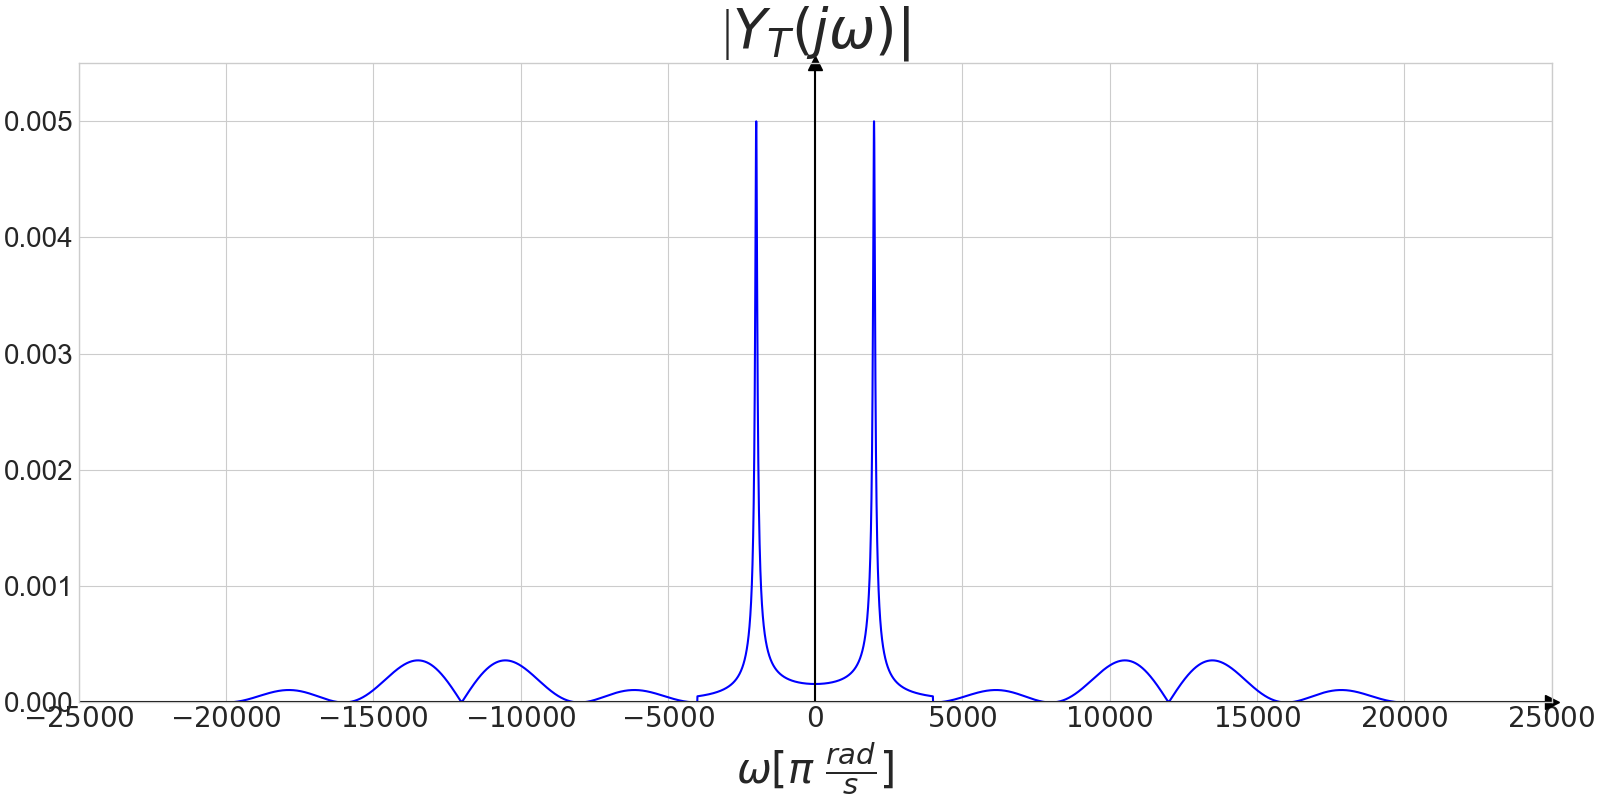
\includegraphics[width=\textwidth]{Images/AmpYT.png}
		\caption{Amplitudski spektar $|Y_T(j\omega)|$}\label{fig:AmpYT}
	\end{figure*}
	\FloatBarrier
	\clearpage
	
	\subsection{Signal $y_R(t)$}
	Signal $y_R(t)$ je signal koji dolazi na drugi kraj kanala veze. Pošto je $\omega_{kv}$ odabrano tako da ne dolazi do gubitka značajnih učestanosti, očekuje se da će signali $y_R(t)$ imati isti amplitudski spektar kao i signal $y_T(t)$. Na sledećoj slici vidimo ovaj spektar:
	\begin{figure*}[ht]
		\centering
		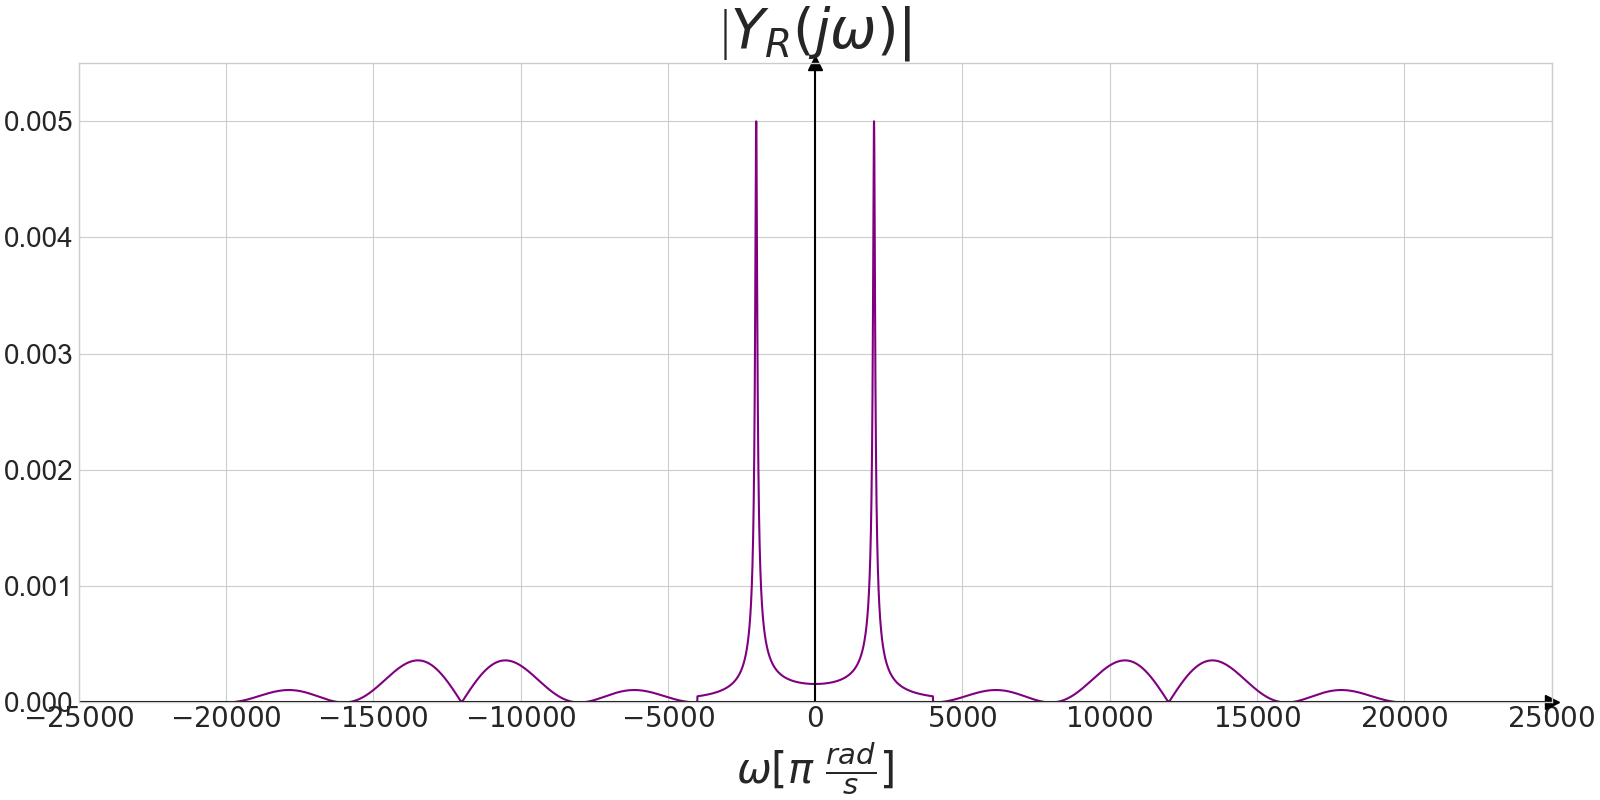
\includegraphics[width=\textwidth]{Images/AmpYR.png}
		\caption{Amplitudski spektar $|Y_R(j\omega)|$}\label{fig:AmpYR}
	\end{figure*}
	\FloatBarrier
	\clearpage
	
	\subsection{Signal $y_2^b(t)$}
	Signal $y_2^b(t)$ dobija se izvdajanjem opsega učestanosti na kojima se prenosi modulisani signal $y_2^m(t)$, odnosno $\omega_{o2d}<|\omega|<\omega_{o2g}$, filtrom $H_{Rb_2}$, iz signala $y_R(t)$. Kako su filtri idealni, ovako filtriran signal biće jednak signalu $y_2^m(t)$. Ovim filtriranjem izvdajaju se učestanosti na kojima se prenosio signal $y_1^n(t)$. Na donjoj slici može se videti amplitudski spektar signala:
	\begin{figure*}[ht]
		\centering
		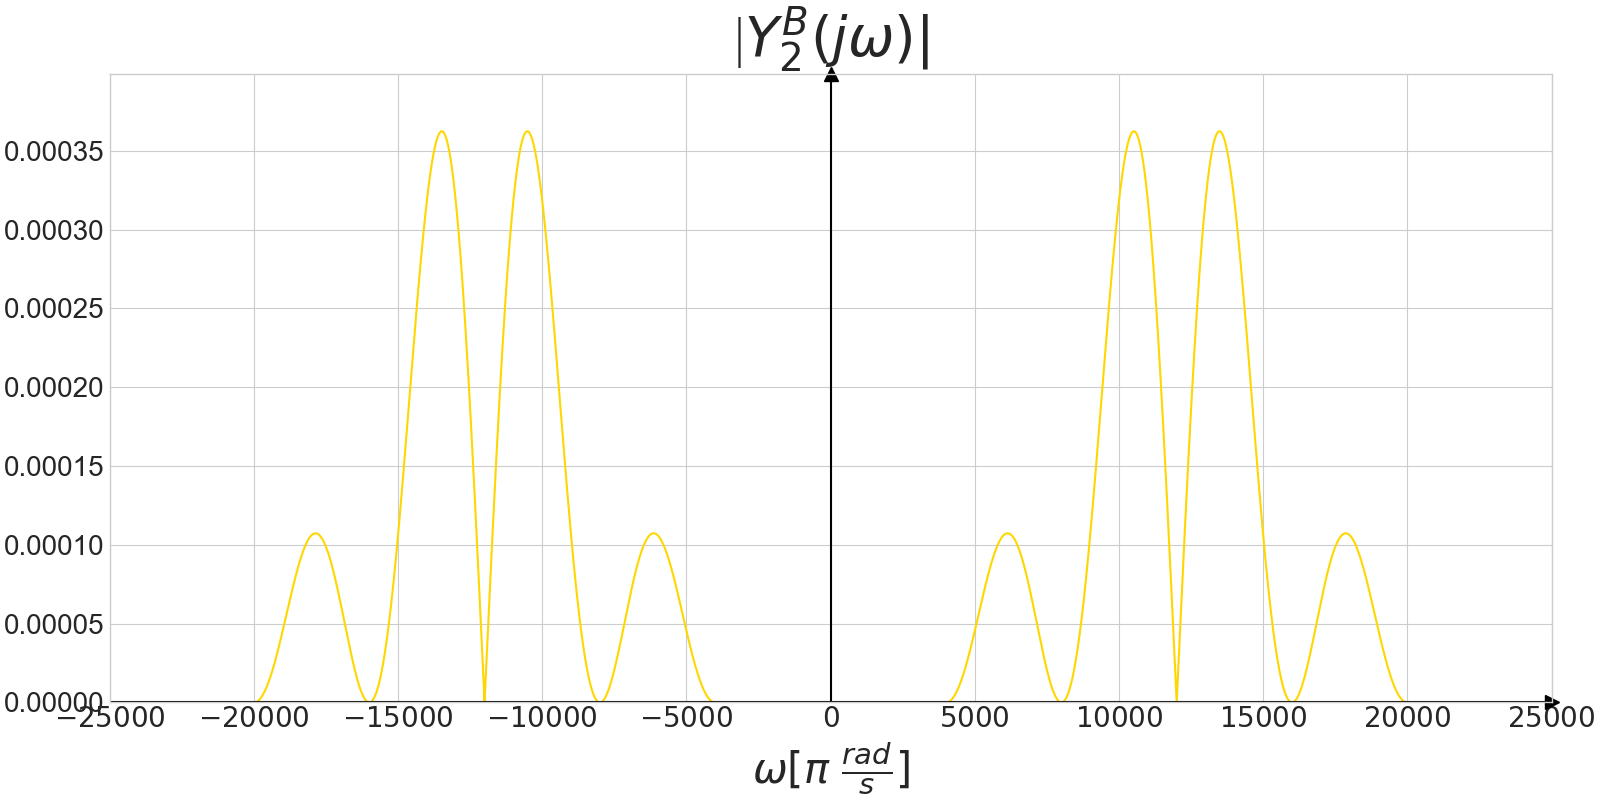
\includegraphics[width=\textwidth]{Images/AmpY2B.png}
		\caption{Amplitudski spektar $|Y_2^B(j\omega)|$}\label{fig:AmpY2B}
	\end{figure*}
	\FloatBarrier
	\clearpage

	\subsection{Signal $y_2^d(t)$}	
	Demodulacijom signala $y_2^b(t)$ sinusoidom $cos(2\pi f_c \cdot t)$, istom kao i pri modulaciji, dobijamo signal $y_2^d(t)$. U vremenskom domenu imamo:
	\begin{equation}
		y_2^d(t) = y_2^b(t)\cdot cos(2\pi f_c \cdot t)
	\end{equation}
	Prelaskom u frekvencijski domen dobijamo:
	\begin{equation}
		Y_2^B(j\omega) = \frac{1}{2\pi}Y_2^D(j\omega)*\mathcal{F}\Big\{cos(2\pi f_c t)\Big\}.
	\end{equation}
	Sličnim postupkom kao i kod signala $y_2^m(t)$, dobijamo izraz za spektar signala $y_2^d(t)$:
	\begin{equation}
		Y_2^D(j\omega) = Y_2^N(j\omega) \frac{1}{2}\Bigg[
		Y_2^N\big(j(\omega-4\pi f_c)\big)+Y_2^N\big(j(\omega+4\pi f_c)\big)
		\Bigg]
	\end{equation}
	Izraz za amplitudski spektar je odavde:
	\begin{gather}
		|Y_2^D(j\omega)| = \left\{
		\begin{array}{rlrr}
			0& \omega \in (&-\infty, &-32000\pi)\\
			\frac{1}{4}|Y_2^N\big(j(\omega+4\pi f_c)\big)|& \omega \in (&-32000\pi,& -16000\pi) \\
			0& \omega \in (&-16000\pi, &-8000\pi) \\
			\frac{1}{2}|Y_2^N\big(j\omega\big)|& \omega \in (&-8000\pi,& 8000\pi) \\
			0& \omega \in (&8000\pi,&16000\pi)\\
			\frac{1}{4}|Y_2^N\big(j(\omega-4\pi f_c)\big)|& \omega \in (&16000\pi,& 32000\pi) \\
			0& \omega \in (&32000\pi,&+\infty)
		\end{array}\right.
	\end{gather}

	Iz formule vidimo da pri drugoj modulaciji, odnosno demodulaciji, u spektru vidimo 3 skalirane kopije spektra početnog signala. Kopija centrirana u $w=0\frac{rad}{s}$ ima amplitudu koja jeduplo manja od amplitude početnog signala, i ovo je deo spektra koji ćemo izvdojiti kao izlazni signal $y_2^r(t)$. U spektru takođe postoje još dve skapirane kopije spektra, sa apitudom koja je četiri puta manja od početne, na učestanostima $w=\pm 24000\pi \frac{rad}{s}$. Ove dve kopije ćemo filtrom $H{d_2r_2}$ ukloniti iz konačnog signala.
	\clearpage
	Na slici ispod može se videti amplitudski spektar signala $y_2^d(t)$.
	\begin{figure*}[ht]
		\centering
		\includegraphics[width=0.9\textwidth]{Images/AmpY2D.png}
		\caption{Amplitudski spektar $|Y_2^D(j\omega)|$}\label{fig:AmpY2D}
	\end{figure*}
	\FloatBarrier
	
	\subsection{Signal $y_1^r(t)$}
	Signal $y_1^r(t)$ dobija se izdvajanjem opsega učestanosti $|\omega|<\omega_{i1}$ filtrom $H_{Rb_1}$ iz signala $y_R(t)$. Ovaj opseg predstavlja spektar signala $y_1^n(t)$ koji je prenošen kao deo signala $y_T(t)$. S obzirom na to da su filtri bili idealni, očekujemo da je signal $y_1^r(t)$ identičan kao i signal $y_1^n(t)$. S obzirom na to da je iz prvobitnog signala $y_1(t)$ vršeno filtriranje viših učestanosti filtrom $H_{n1}$, ove učestanosti nisu prisutne u spektru signala $y_1^r(t)$, što znači da se signali $y_1(t)$ i $y_1^r(t)$ razlikuju. Može se izvesti formula za vemenski oblik signala $y_1^r(t)$:
	\begin{equation}
		y_1^r(t) = \frac{1}{2\pi}\int_{-\omega_{i1}}^{\omega_{i1}}Y_1^N(j\omega)e^{j\omega t}d\omega,
	\end{equation}
	ali kako se integral ne može analitički odrediti, vremenski oblik signala nije prikazan.
	
	\clearpage
	
	\subsection{Signal $y_2^r(t)$}
	Signal $y_2^r(t)$ dobija se propuštanjem signala $y_2^d(t)$ kroz filtar $H_{d_2r_2}$. Ovime se izdvajaju skapirane kopije spektra na učestanostima $\pm 4\pi f_c$, nastale modulacijom i demodulacijom. Za rezultujući spektar važi:
	\begin{gather}
		Y_2^R(j\omega) = \frac{1}{2} Y_2^N(j\omega)
		|Y_2^R(j\omega)| = \frac{1}{2}|Y_2^N(j\omega)|.
	\end{gather}
	
	Iz prethodno izvedenih jednačina faznih spektara ostalih signala, vidimo da će amplituda prenošenog signala $y_2^n(t)$ biti dva puta manja usled procesa filtriranja, modulacije i demodulacije. Vremenski oblik može se pronaći sličnim postupkom kao i kod signala $y_2^r(t)$, ali je izostavljen jer ni ovaj integral nije analitički rešiv. Na sledećoj slici može se videti amplitudski spektar signala $y_2^r(t)$.
	\begin{figure*}[ht]
		\centering
		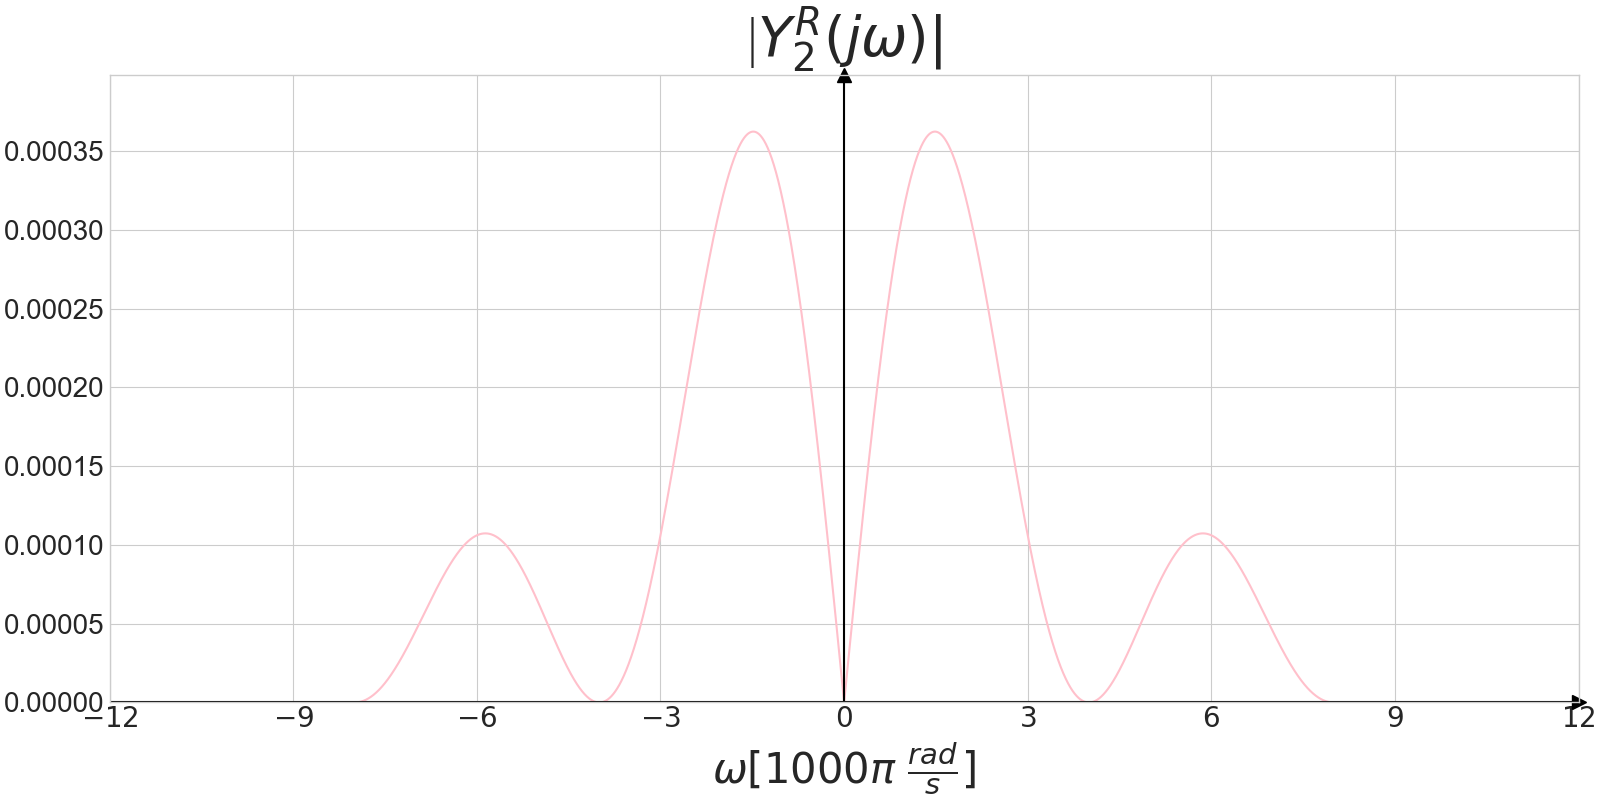
\includegraphics[width=0.8\textwidth]{Images/AmpY2R.png}
		\caption{Amplitudski spektar $|Y_2^R(j\omega)|$}\label{fig:AmpY2R}
	\end{figure*}
	\FloatBarrier
	\pagebreak
	\clearpage
	
	\section{Rekonstruisani signali}
	Treba analizirati kako izgledaju signali $y_1^r(t)$ i $y_2^r(t)$ u odnosu na signale koji su početno transmitovani, $y_1(t)$ i $y_2(t)$.
	
	Signal $y_1^r(t)$, u odnosu na signal $y_1(t)$, zadržava amplitudu, ali u njemu, usled filtracija koje su vršene u Sistemu. nedostaju visoke učestanosti. U spektru se ovo oslikava nultim vrednostima amplitude za visoke učestanosti, dok se u vremenu mogu očekivati izobličenja signala.
	
	Signal  $y_2^r(t)$ u odnosu na signal $y_2(t)$ ima duplo manju amplitudu. Ovo se dešava usled procesa modulacije i demodulacije signala u okviru Sistema. Kao i kod signala $y_1^r(t)$, i u ovom signalu nedostaju visoke učestanosti, i očekivana su izobličenja u odnosu na početni signal.
	
	\section{Kodovi za generisanje grafika}
	Za crtanje grafika korišćen je programski jezik \textbf{Python} i biblioteke \emph{matplotlib} i \emph{numpy}. Za repetativni deo koda napisane su dve klase koje olakšavaju crtanje pojedinačnih karakteristika. Postoje i dva fajla u kojima se nalaze sve funkcije koje su grafički predstavljanje.
	
	\bigskip
	\noindent Kod kalsa za crtanje funkcija po zadatim vrednostima:
	\lstinputlisting[language=Python, caption={drawer.py}]{Codes/drawer.py}
	Kod pomocnih funkcija:
	\lstinputlisting[language=Python, caption={functions.py}]{Codes/functions.py}
	Kod pomocnih funkcija - signala:
	\lstinputlisting[language=Python, caption={signals.py}]{Codes/signals.py}
	Kod za crtanje amplitudske karakteristike $Y_1(j\omega)$: 
	\lstinputlisting[language=Python, caption={AmpY1.py}]{Codes/AmpY1.py}
	Kod za crtanje amplitudske karakteristike $Y_2(j\omega):$ 
	\lstinputlisting[language=Python, caption={AmpY2.py}]{Codes/AmpY2.py}
	Kod za crtanje amplitudske karakteristike $Y_1^N(j\omega):$ 
	\lstinputlisting[language=Python, caption={AmpY1N.py}]{Codes/AmpY1N.py}
	Kod za crtanje amplitudske karakteristike $Y_2^N(j\omega):$ 
	\lstinputlisting[language=Python, caption={AmpY2N.py}]{Codes/AmpY2N.py}
	Kod za crtanje amplitudske karakteristike $Y_2^M(j\omega):$ 
	\lstinputlisting[language=Python, caption={AmpY2M.py}]{Codes/AmpY2M.py}
	Kod za crtanje amplitudske karakteristike $Y_T(j\omega):$ 
	\lstinputlisting[language=Python, caption={AmpYT.py}]{Codes/AmpYT.py}
	Kod za crtanje amplitudske karakteristike $Y_R(j\omega):$ 
	\lstinputlisting[language=Python, caption={AmpYR.py}]{Codes/AmpYR.py}
	Kod za crtanje amplitudske karakteristike $Y_2^B(j\omega):$ 
	\lstinputlisting[language=Python, caption={AmpY2B.py}]{Codes/AmpY2B.py}
	Kod za crtanje amplitudske karakteristike $Y_2^D(j\omega):$ 
	\lstinputlisting[language=Python, caption={AmpY2D.py}]{Codes/AmpY2D.py}
	Kod za crtanje amplitudske karakteristike $Y_2^R(j\omega):$ 
	\lstinputlisting[language=Python, caption={AmpY2R.py}]{Codes/AmpY2R.py}
	

	\clearpage
	\lstlistoflistings
	
\end{document}
